% ============================================================
\chapter{Equivariant and Invariant Networks}
\label{ch:equivariant}
% ============================================================

Convolutional neural networks owe their success to a precise mathematical property: translation equivariance. A cat remains a cat, whether it sits on the left or right of the image. But what happens when the relevant symmetries are not translations? In molecular chemistry, a molecule's properties are invariant under rotation and translation of all its atoms. In particle physics, interactions obey gauge symmetries. Taco Cohen and Max Welling, in 2016, pioneered \emph{equivariant networks} by showing how to build neural network layers that respect the symmetries of a given group. This approach, formalized by the geometric framework of Bronstein et al., unifies CNNs, GNNs, and transformers as special cases of a single principle: the network's structure must reflect the problem's symmetries.

\section{General Formalism}

\subsection{Equivariance Review}

\begin{definition}[General equivariance]
Let $G$ be a group acting on spaces $\mathcal{X}$ and $\mathcal{Y}$ via
representations $\rho_{\mathcal{X}}$ and $\rho_{\mathcal{Y}}$. A function
$f: \mathcal{X} \to \mathcal{Y}$ is \textbf{$G$-equivariant} if:
\[
    f(\rho_{\mathcal{X}}(g) \cdot x) = \rho_{\mathcal{Y}}(g) \cdot f(x),
    \quad \forall g \in G,\; \forall x \in \mathcal{X}.
\]
\end{definition}

\begin{proposition}[Composition of equivariant maps]
If $f: \mathcal{X} \to \mathcal{Y}$ and $g: \mathcal{Y} \to \mathcal{Z}$ are
equivariant, then $g \circ f: \mathcal{X} \to \mathcal{Z}$ is equivariant.
This justifies stacking equivariant layers in a deep network.
\end{proposition}

\subsection{Constructing Equivariant Layers}

\begin{theorem}[Characterization of equivariant linear layers]
The space of $G$-equivariant linear maps $T: V \to W$ is:
\[
    \mathrm{Hom}_G(V, W) = \{T \in \mathrm{Lin}(V, W) :
    T \rho_V(g) = \rho_W(g) T,\; \forall g \in G\}
\]
Its dimension is given by the inner product of characters:
$\dim \mathrm{Hom}_G(V, W) = \inner{\chi_V}{\chi_W}_G$.
\end{theorem}

\begin{intuition}[title=\textbf{Equivariance constraint = weight sharing}]
Imposing equivariance amounts to \textbf{constraining the weight matrix} of
the linear layer. The larger the symmetry group, the stronger the constraint,
and the fewer free parameters.
\begin{center}
\begin{tabular}{lll}
\toprule
\textbf{Group} & \textbf{Constraint} & \textbf{Parameters} \\
\midrule
Trivial $\{e\}$ & None & $n^2$ \\
Translation $\Z^d$ & Toeplitz (convolution) & $k^d$ \\
Permutation $S_n$ & Doubly stochastic & $2$ \\
$\mathrm{SO}(3)$ & Clebsch--Gordan & $\sum_k n_k m_k$ \\
\bottomrule
\end{tabular}
\end{center}
\end{intuition}

\section{$\mathrm{SE}(3)$-Equivariant Networks}

\subsection{Motivation: Physics and Chemistry}

Many physical problems possess $\mathrm{SE}(3)$ symmetry (rotations +
translations):
\begin{itemize}
    \item Molecular energy prediction.
    \item Protein dynamics.
    \item Fluid simulation.
\end{itemize}

\subsection{Type-$\ell$ Representations}

\begin{definition}[Type-$\ell$ tensor fields]
A \textbf{type-$\ell$ tensor field} is a function
$f: \R^3 \to \R^{2\ell+1}$ that transforms according to the irreducible
representation $D^\ell$ under rotation:
\[
    [L_R f](\mathbf{x}) = D^\ell(R)\, f(R^{-1}\mathbf{x})
\]
\begin{itemize}
    \item $\ell = 0$: scalars (1D)---energy, charge.
    \item $\ell = 1$: vectors (3D)---forces, velocities.
    \item $\ell = 2$: order-2 traceless tensors (5D)---stresses.
\end{itemize}
\end{definition}

\subsection{Tensor Field Networks (TFN)}

\begin{definition}[TFN --- Thomas et al., 2018]
\textbf{Tensor Field Networks} define $\mathrm{SE}(3)$-equivariant layers
using tensor products of irreducible representations. For a node $v$ at
position $\mathbf{r}_v$:
\[
    \mathbf{h}_v^{\ell, (\text{out})} = \sum_{\ell_1, \ell_2}
    \sum_{u \in \mathcal{N}(v)} W^{\ell_1 \ell_2 \ell}(r_{vu})\,
    \left(\mathbf{h}_u^{\ell_1} \otimes_{\text{CG}} Y^{\ell_2}(\hat{\mathbf{r}}_{vu})\right)^\ell
\]
where:
\begin{itemize}
    \item $\hat{\mathbf{r}}_{vu} = (\mathbf{r}_v - \mathbf{r}_u) / r_{vu}$ is
          the normalized direction.
    \item $Y^{\ell_2}(\hat{\mathbf{r}})$ are spherical harmonics.
    \item $\otimes_{\text{CG}}$ is the tensor product with Clebsch--Gordan
          coefficients.
    \item $W^{\ell_1 \ell_2 \ell}(r)$ is a radial kernel (scalar, hence invariant).
\end{itemize}
\end{definition}

\begin{theorem}[TFN equivariance]
TFN layers are $\mathrm{SE}(3)$-equivariant: for $R \in \mathrm{SO}(3)$ and
$\mathbf{t} \in \R^3$:
\[
    f(R\mathbf{r}_1 + \mathbf{t}, \ldots, R\mathbf{r}_n + \mathbf{t})
    = \bigoplus_\ell D^\ell(R)\, f(\mathbf{r}_1, \ldots, \mathbf{r}_n)
\]
The proof relies on the transformation property of spherical harmonics and
the Clebsch--Gordan decomposition.
\end{theorem}

\begin{codeblock}[title=\textbf{Equivariant network with e3nn}]
\begin{minted}{python}
import torch
from e3nn import o3
from e3nn.nn.models.gate_points_2101 import Network

model = Network(
    irreps_in="5x0e",
    irreps_hidden="32x0e + 8x1o + 4x2e",
    irreps_out="1x0e",  # scalar output (energy)
    irreps_node_attr="1x0e",
    irreps_edge_attr=o3.Irreps.spherical_harmonics(lmax=2),
    layers=3,
    max_radius=5.0,
    number_of_basis=10,
    radial_layers=2,
    radial_neurons=64,
    num_neighbors=12,
    num_nodes=20,
)

positions = torch.randn(20, 3)
node_features = torch.randn(20, 5)
node_attrs = torch.ones(20, 1)

# Verify equivariance
R = o3.rand_matrix()
out_original = model({"node_input": node_features,
                       "positions": positions,
                       "node_attrs": node_attrs})
out_rotated = model({"node_input": node_features,
                      "positions": positions @ R.T,
                      "node_attrs": node_attrs})
print(f"Scalar invariance: "
      f"{torch.allclose(out_original, out_rotated, atol=1e-4)}")
\end{minted}
\end{codeblock}

\section{EGNN: Simplified Equivariance}

\begin{definition}[EGNN --- Satorras et al., 2021]
\textbf{E(n) Equivariant Graph Neural Networks} (EGNN) achieve
$\mathrm{E}(n)$ equivariance \textbf{without} irreducible representations:
\begin{align}
    \mathbf{m}_{ij} &= \phi_e(\mathbf{h}_i, \mathbf{h}_j, d_{ij}^2, a_{ij}) \\
    \mathbf{h}_i' &= \phi_h\!\left(\mathbf{h}_i, \sum_{j \neq i} \mathbf{m}_{ij}\right) \\
    \mathbf{x}_i' &= \mathbf{x}_i + \sum_{j \neq i} (\mathbf{x}_i - \mathbf{x}_j)\,
    \phi_x(\mathbf{m}_{ij})
\end{align}
where $d_{ij} = \norm{\mathbf{x}_i - \mathbf{x}_j}$ and $\phi_e, \phi_h, \phi_x$
are MLPs.
\end{definition}

\begin{proposition}[EGNN equivariance]
\begin{enumerate}
    \item \textbf{Scalar features} $\mathbf{h}_i$ are \textbf{invariant} under
          $\mathrm{E}(n)$.
    \item \textbf{Coordinates} $\mathbf{x}_i$ are \textbf{equivariant} under
          $\mathrm{E}(n)$.
    \item The proof relies on $d_{ij}^2$ and $\mathbf{x}_i - \mathbf{x}_j$
          transforming correctly.
\end{enumerate}
\end{proposition}

\begin{codeblock}[title=\textbf{EGNN implementation}]
\begin{minted}{python}
import torch
import torch.nn as nn

class EGNNLayer(nn.Module):
    """E(n) equivariant layer."""
    def __init__(self, node_dim, hidden_dim):
        super().__init__()
        self.phi_e = nn.Sequential(
            nn.Linear(2 * node_dim + 1, hidden_dim),
            nn.SiLU(),
            nn.Linear(hidden_dim, hidden_dim),
        )
        self.phi_h = nn.Sequential(
            nn.Linear(node_dim + hidden_dim, hidden_dim),
            nn.SiLU(),
            nn.Linear(hidden_dim, node_dim),
        )
        self.phi_x = nn.Sequential(
            nn.Linear(hidden_dim, hidden_dim),
            nn.SiLU(),
            nn.Linear(hidden_dim, 1),
        )

    def forward(self, h, x, edge_index):
        row, col = edge_index
        diff = x[row] - x[col]
        dist_sq = (diff ** 2).sum(dim=-1, keepdim=True)
        m = self.phi_e(torch.cat([h[row], h[col], dist_sq], dim=-1))
        agg = torch.zeros_like(h)
        agg.index_add_(0, row, m)
        h_new = h + self.phi_h(torch.cat([h, agg], dim=-1))
        x_weights = self.phi_x(m)
        x_agg = torch.zeros_like(x)
        x_agg.index_add_(0, row, diff * x_weights)
        x_new = x + x_agg
        return h_new, x_new

# Equivariance test
layer = EGNNLayer(32, 64)
h = torch.randn(10, 32)
x = torch.randn(10, 3)
edge_index = torch.randint(0, 10, (2, 30))

h_out, x_out = layer(h, x, edge_index)

R = torch.linalg.qr(torch.randn(3, 3))[0]
if R.det() < 0:
    R[:, 0] *= -1
h_rot, x_rot = layer(h, x @ R.T, edge_index)
print(f"h invariant: {torch.allclose(h_out, h_rot, atol=1e-4)}")
print(f"x equivariant: {torch.allclose(x_out @ R.T, x_rot, atol=1e-4)}")
\end{minted}
\end{codeblock}

\section{Invariant Networks}

\begin{definition}[Fundamental invariants]
To build an $\mathrm{E}(n)$-invariant network, one can use
\textbf{fundamental invariants}:
\begin{enumerate}
    \item \textbf{Distances}: $d_{ij} = \norm{\mathbf{x}_i - \mathbf{x}_j}$.
    \item \textbf{Angles}: $\theta_{ijk} = \arccos\!\left(\frac{(\mathbf{x}_j - \mathbf{x}_i) \cdot
          (\mathbf{x}_k - \mathbf{x}_i)}{\norm{\mathbf{x}_j - \mathbf{x}_i}\norm{\mathbf{x}_k - \mathbf{x}_i}}\right)$.
    \item \textbf{Dihedral}: angle between planes defined by $(i,j,k)$ and $(j,k,l)$.
\end{enumerate}
\end{definition}

\begin{theorem}[Completeness of invariants]
Interatomic distances $\{d_{ij}\}$ determine the geometry up to reflection.
Adding dihedral angles resolves the reflection ambiguity. Every $\mathrm{SE}(3)$
invariant can be expressed as a function of distances and angles.
\end{theorem}

\begin{definition}[SchNet --- Sch\"utt et al., 2018]
SchNet uses interatomic distances as the sole geometric information:
\[
    \mathbf{h}_i^{(\ell+1)} = \mathbf{h}_i^{(\ell)} + \sum_{j \in \mathcal{N}(i)}
    \mathbf{W}^{(\ell)} \mathbf{h}_j^{(\ell)} \odot \text{RBF}(d_{ij})
\]
where $\text{RBF}(d) = [\exp(-\gamma_1(d - \mu_1)^2), \ldots, \exp(-\gamma_K(d - \mu_K)^2)]$
is a radial basis function expansion.
\end{definition}

\section{Hierarchy of Equivariant Models}

\begin{figure}[htbp]
\centering
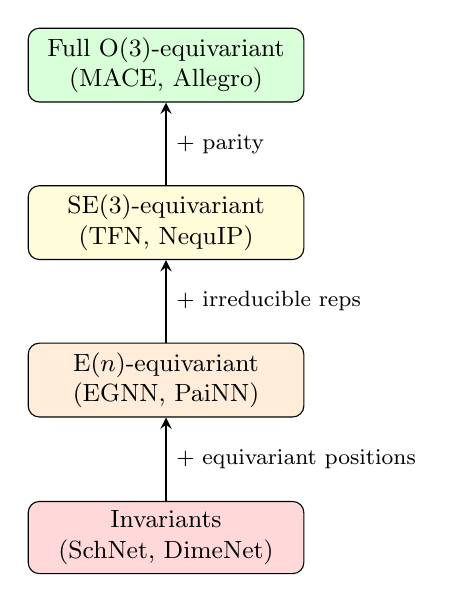
\begin{tikzpicture}[
    box/.style={rectangle, draw, rounded corners, fill=#1!15,
                minimum width=3.5cm, minimum height=0.9cm, align=center,
                font=\small},
    arr/.style={->, thick, >=stealth}
]
\node[box=red] (inv) at (0, 0) {Invariants\\(SchNet, DimeNet)};
\node[box=orange] (e3) at (0, 2) {$\mathrm{E}(n)$-equivariant\\(EGNN, PaiNN)};
\node[box=yellow] (se3) at (0, 4) {$\mathrm{SE}(3)$-equivariant\\(TFN, NequIP)};
\node[box=green] (full) at (0, 6) {Full $\mathrm{O}(3)$-equivariant\\(MACE, Allegro)};

\draw[arr] (inv) -- node[right, font=\footnotesize] {+ equivariant positions} (e3);
\draw[arr] (e3) -- node[right, font=\footnotesize] {+ irreducible reps} (se3);
\draw[arr] (se3) -- node[right, font=\footnotesize] {+ parity} (full);
\end{tikzpicture}
\caption{Hierarchy of equivariant architectures.}
\end{figure}

\section*{Exercises}

\begin{exercise}[Equivariance verification]
For each of the following models, numerically verify equivariance by applying
random rotations, translations, and reflections:
\begin{enumerate}
    \item SchNet ($\mathrm{E}(3)$ invariance).
    \item EGNN ($\mathrm{E}(n)$ equivariance).
    \item A TFN with vector outputs ($\mathrm{SE}(3)$ equivariance).
\end{enumerate}
\end{exercise}

\begin{exercise}[Tensor products]
\begin{enumerate}
    \item Compute the tensor product $1 \otimes 1$ for $\mathrm{SO}(3)$ and
          verify $D^1 \otimes D^1 = D^0 \oplus D^1 \oplus D^2$.
    \item Implement with \texttt{e3nn} and verify.
    \item Build an equivariant layer that takes two vectors and produces a
          scalar (dot product), a vector (cross product), and an order-2 tensor.
\end{enumerate}
\end{exercise}

\begin{exercise}[EGNN from scratch]
Implement a complete EGNN for molecular energy prediction on the QM9 dataset.
\begin{enumerate}
    \item Load QM9 from PyTorch Geometric.
    \item Implement 4 EGNN layers.
    \item Train on the $U_0$ property (internal energy).
    \item Verify $\mathrm{E}(3)$ invariance of predictions.
\end{enumerate}
\end{exercise}

\begin{exercise}[Invariant vs.\ equivariant comparison]
Compare SchNet (invariant) and EGNN (equivariant) on molecular force prediction
(a vectorial quantity).
\begin{enumerate}
    \item Why can SchNet not directly predict forces?
    \item How are forces obtained from an energy model?
    \item Does EGNN directly predict equivariant forces?
\end{enumerate}
\end{exercise}
